%                      Code_Saturne version 1.3
%                      ------------------------
%
%     This file is part of the Code_Saturne Kernel, element of the
%     Code_Saturne CFD tool.
% 
%     Copyright (C) 1998-2007 EDF S.A., France
%
%     contact: saturne-support@edf.fr
% 
%     The Code_Saturne Kernel is free software; you can redistribute it
%     and/or modify it under the terms of the GNU General Public License
%     as published by the Free Software Foundation; either version 2 of
%     the License, or (at your option) any later version.
% 
%     The Code_Saturne Kernel is distributed in the hope that it will be
%     useful, but WITHOUT ANY WARRANTY; without even the implied warranty
%     of MERCHANTABILITY or FITNESS FOR A PARTICULAR PURPOSE.  See the
%     GNU General Public License for more details.
% 
%     You should have received a copy of the GNU General Public License
%     along with the Code_Saturne Kernel; if not, write to the
%     Free Software Foundation, Inc.,
%     51 Franklin St, Fifth Floor,
%     Boston, MA  02110-1301  USA
%
%-----------------------------------------------------------------------
%

\programme{clptur}

\vspace{1cm}
%%%%%%%%%%%%%%%%%%%%%%%%%%%%%%%%%%
%%%%%%%%%%%%%%%%%%%%%%%%%%%%%%%%%%
\section{Fonction}
%%%%%%%%%%%%%%%%%%%%%%%%%%%%%%%%%%
%%%%%%%%%%%%%%%%%%%%%%%%%%%%%%%%%%
Ce sous-programme est d\'edi\'e au calcul des conditions aux limites en paroi. 
On utilise le formalisme introduit dans \var{CONDLI} pour les conditions
aux limites g\'en\'erales. 

Par conditions aux limites en paroi, on entend ici l'ensemble des conditions aux
limites pour la vitesse, les grandeurs turbulentes ($k$, $\varepsilon$,
$R_{ij}$), la temp\'erature lorsqu'elle a une valeur de paroi impos\'ee  
(ou l'enthalpie et plus g\'en\'eralement les 
{\it VarScalaires}\footnote{Comme dans \fort{condli}, on d\'esignera ici par 
{\it VarScalaire} toute variable solution
d'une \'equation de convection-diffusion autre que la 
vitesse, la pression et les grandeurs turbulentes $k$, $\varepsilon$ et
$R_{ij}$. La d\'enomination {\it VarScalaire} pourra en particulier se rapporter
\`a la temp\'erature, \`a l'enthalpie ou \`a un scalaire passif.} 
\`a traiter en paroi en prenant en compte une loi de similitude
pour la couche limite associ\'ee). Pour les {\it VarScalaires}, en particulier,
lorsque les conditions aux limites de paroi sont du type Neumann (homog\`ene ou non),
elles sont trait\'ees dans \fort{condli} et on ne s'y int\'eresse donc pas
ici. En particulier, les conditions aux limites des  {\it VarScalaires}
repr\'esentant la variance de fluctuations d'autres  {\it VarScalaires} ne
sont pas trait\'ees ici car leur traitement en paroi est de type Neumann homog\`ene. 

On indique comment sont calcul\'es les couples de coefficients 
$A_b$ et $B_b$ qui sont utilis\'es pour le calcul de certains 
termes discrets des \'equations \`a r\'esoudre et qui
permettent  en particulier de d\'eterminer une valeur associ\'ee aux faces 
de bord $f_{b,int}$ (en un point localis\'e au ``centre'' de la face de bord, 
barycentre de ses sommets) par la
relation $f_{b,int} = A_b+B_b\,f_{I'}$ ($f_{I'}$ est la valeur de 
la variable au point
$I'$, projet\'e du centre de la cellule jouxtant le bord sur la droite 
normale \`a 
la face de bord et passant par son centre~: voir la figure~\ref{Base_Clptur_fig_flux_clptur}). 

\begin{figure}[h]
\centerline{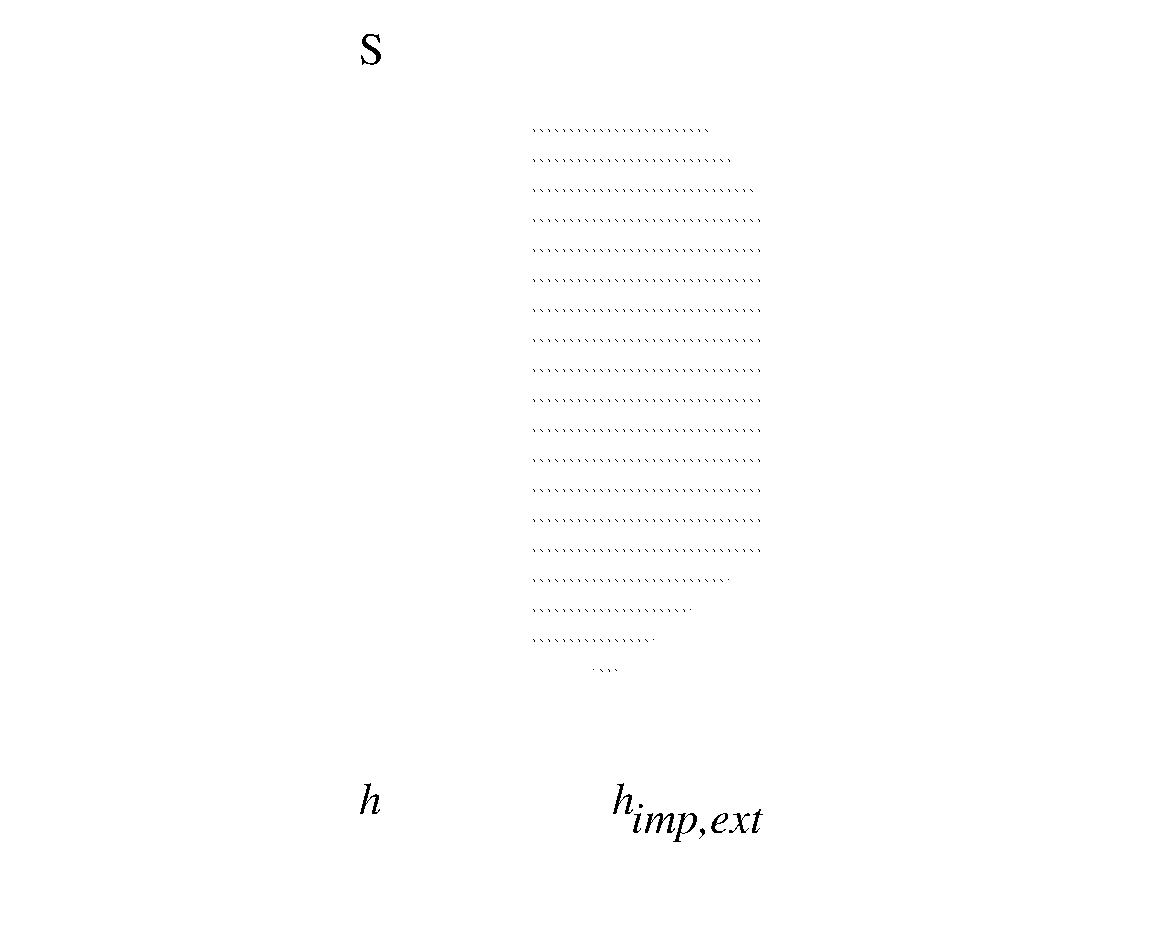
\includegraphics[height=7cm]{../Base/Clptur/Images/fluxbord.pdf}}
\caption{\label{Base_Clptur_fig_flux_clptur}Cellule de bord.}
\end{figure}
